%%%%%%%%%%%%%%%%%%%%%%%%%%%%%%%%%%%%%%%%%%%%%%%%%%%%%%%%%%%%%%%%%%%%%%%%%%%%%%%%
%2345678901234567890123456789012345678901234567890123456789012345678901234567890
%        1         2         3         4         5         6         7         8
% Things to do tonight:
% Enumerate thigns that audience needs to understand in background
% What do they need to understand to make sense of markov categories?
% Enumerate the string diagrams that they'll need to understand to make sense of the string diagram for the KF
% Generate those string diagrams
\documentclass[letterpaper, 10 pt, conference]{ieeeconf}  % Comment this line out if you need a4paper

%\documentclass[a4paper, 10pt, conference]{ieeeconf}      % Use this line for a4 paper

\IEEEoverridecommandlockouts                              % This command is only needed if 
                                                          % you want to use the \thanks command

\overrideIEEEmargins                                      % Needed to meet printer requirements.

%In case you encounter the following error:
%Error 1010 The PDF file may be corrupt (unable to open PDF file) OR
%Error 1000 An error occurred while parsing a contents stream. Unable to analyze the PDF file.
%This is a known problem with pdfLaTeX conversion filter. The file cannot be opened with acrobat reader
%Please use one of the alternatives below to circumvent this error by uncommenting one or the other
%\pdfobjcompresslevel=0
%\pdfminorversion=4

% See the \addtolength command later in the file to balance the column lengths
% on the last page of the document

% The following packages can be found on http:\\www.ctan.org
%\usepackage{graphics} % for pdf, bitmapped graphics files
%\usepackage{epsfig} % for postscript graphics files
%\usepackage{mathptmx} % assumes new font selection scheme installed
%\usepackage{times} % assumes new font selection scheme installed
%\usepackage{amsmath} % assumes amsmath package installed
%\usepackage{amssymb}  % assumes amsmath package installed
\usepackage{standalone}
\usepackage{freetikz}
\usepackage{tikz-cd}
\usepackage{biblatex}
\usepackage{minted}
\usepackage{xcolor} % to access the named colour LightGray
\definecolor{LightGray}{gray}{0.9}
\addbibresource{bibliography.bib}

\title{\LARGE \bf
Toward Synthetic Algorithms for Stochastic Systems
}


\author{Drew McNeely$^{1}$ and Jeffrey Cochran$^{2}$ and Efstathios Bakolas$^{1}$% <-this % stops a space
\thanks{$^{1}$Drew McNeely and Efstathios Bakolas are with Department of Aerospace Engineering, 
        The University of Texas at Austin, 2617 Wichita St., Austin, TX 78712
        {\tt\small drew.mcneely@utexas.edu, bakolas@austin.utexas.edu}}%
\thanks{$^{2}$Jeffrey Cochran is with the Oden Institute for Computational Engineering and Sciences, The University of Texas at Austin, 201 E. 24th St., Austin, TX 78712
        Dayton, OH 45435, USA
        {\tt\small jeffrey.david.cochran@utexas.edu}}%
}


\begin{document}



\maketitle
\thispagestyle{empty}
\pagestyle{empty}


%%%%%%%%%%%%%%%%%%%%%%%%%%%%%%%%%%%%%%%%%%%%%%%%%%%%%%%%%%%%%%%%%%%%%%%%%%%%%%%%
\begin{abstract}
The tracking community has been inundated with variations on the same themes. Kalman filters beget extended Kalman filters, beget unscented Kalman filters. Each variation adds complexity to the derivation of the resulting algorithm, which must change to accommodate new assumptions. This paper unifies these algorithms under a single, simple abstract implementation. The framework developed for this purpose enables the fast and intuitive extension of these algorithms to new and more complicated assumptions. We present this new framework and briefly summarize the mathematical background necessary to understand the it. We demonstrate the simplicity that this framework offers by way of a few examples, and we confirm that our new, unifying implementation does in fact reproduce the expected results. We conclude by discussing the exciting work on the horizon. 

\end{abstract}


%%%%%%%%%%%%%%%%%%%%%%%%%%%%%%%%%%%%%%%%%%%%%%%%%%%%%%%%%%%%%%%%%%%%%%%%%%%%%%%%
\section{INTRODUCTION}

The tracking community has been inundated with variations on the same themes. Kalman filters beget extended Kalman filters, beget unscented Kalman filters. Each variation adds complexity to the derivation of the resulting algorithm, which must change to accommodate new assumptions. This paper unifies these algorithms under a single, simple abstract implementation. The framework developed for this purpose enables the fast and intuitive extension of these algorithms to new and more complicated assumptions. We present this new framework and briefly summarize the mathematical background necessary to understand the it. We demonstrate the simplicity that this framework offers by way of a few examples, and we confirm that our new, unifying implementation does in fact reproduce the expected results. We conclude by discussing the exciting work on the horizon.

The notion of abstracting an algorithm is ubiquitous, and only the inability to conceive of a unifying description has prevented doing so for Kalman filters and other algorithms on stochastic systems. 

POSETS and sorting algorithms.

The only unifying description that we've had so far is PDFs, which is incompatible with computation. Algorithms should not rely on a specific representation of the probability distributions in question to work; the underlying idea is unchanged. One should be able work with the parameterization of a PDF just as well as one might work with the numerical represenation of the PDF.

Not only this, but we conjecture that the framework we propose is not restricted to the classic notion of measure theoretic probabilities, but also encompasses possibilities, information, and outer probability measures \cite{delande}. 

\subsection{Literature Review}

THE OLD PAPER THAT TALKS ABOUT IMPLICIT CONVERSIONS AND GENERIC OPERATORS

The foundations of this work stem from the research of Fritz \cite{fritz}, who in turn builds on the work of Cho and Jacobs \cite{cho} and others.

Cho and Jacobs first defined Markov categories (then called CD-categories) as used to describe generic stochastic transition maps and described their manipulation in terms of string diagrams. Fritz then greatly generalized this work, introducing the name "Markov category" and giving several abstract examples of Markov categories built synthetically. 

Baez and Erbele \cite{baez} actually preceded these works with a description of deterministic controls in terms of string diagrams. Here they add relational structure to the monoidal categories of dynamical system configuration spaces in order to redescribe the \emph{block diagrams} used pervasively in controls in terms of a string diagram language that is more amenable to computation.
This work gives exciting avenues for future research, and we plan to incorporate this description into stochastic systems.

Other filtering papers that work without reference to category theory employ an impressive toolbox that, in hindsight, very evidently use concepts that are generalized in the categorical viewpoint of filtering.
Menegaz et al.\ \cite{menegaz} generalize Unscented Kalman Filters to Riemannian manifolds, and they very clearly build joint probability manifold-spaces in ways that can be easily described with monoidal categories.
We propose that our framework will contribute somewhat to simplifying the description and implementation of algorithms such as this.


\subsection{Contribution}
1. actual framework (software)
2. expressing kalman filter in category theoretical terms
3. demonstrating how this expression of the kalman filter enables intuitive extensions and implementations

\section{PRELIMINARIES}

While it is extremely helpful to the reader to understand certain concepts in category theory and functional programming, it isn't strictly required.

Ideas:
This research doesn't focus on creating generic categories in software but rather specifying the requirements for creating Markov categories specifically.
In the context of software, Markov categories can be thought of as collections of stochastic transition kernels going between spaces.
When implementing a data type, one needs to consider a family of spaces to represent configurations and what stochastic transition kernels between those spaces look like.
Categorical probability theory focuses less on what probability distributions/stochastic maps are comprised of, and more on how they behave with respect to each other.

Things that people need to understand:
The definition of a stochastic kernel
How stochastic kernels compose, even though their underlying types don't line up
How distributions can be represented as kernels coming out of the singleton
	This isn't exactly necessary and may add to the boilerplate, but it allows composition to do double duty as a distribution pushforwarder as well
The 7 basic methods required of stochastic kernels
String diagrams
Abstract classes, interfaces, and/or typeclasses
Higher order functions
infix operators in python?

\subsection{Notation}

whatever you need to understand a string diagram and your infix notation

\subsection{Concepts in Category Theory}

whatever they need to understand a markov category

As stated above, a thorough understanding of category theory is not strictly necessary to make sense of this.
The basic idea in categorical probability theory is that Markov categories have in some sense a minimal set of axioms necessary to specify how stochastic transition kernels and distributions behave.
One thing to note is that a categorical framework that works with markov maps is not limited to Markov systems.
One can build up more general systems as Markov transitions into joint history spaces.

In short, a category is a possibly infinite directed graph in which the edges have an algebra of paths that describe associative composition and identity.
For details, we invite the reader to explore a wide ranging library of literature covering category theory, widely ranging in entertainment value \cite{bartosz}\cite{context}.
While this abstract definition works, its obtuse nature can make the topic difficult to approach and render its relevance opaque.
In most concrete applications, the langauge of categories can be successfully used to describe families of spaces with a certain structure (represented by objects, ie. the graph's nodes) and structure preserving transformations between them (represented by the edges or morphisms as they're known).
We can make an important observation about this construction: a category is concerned less with what elements structured spaces are composed of and more with how they behave around their neighbors.
In other words, while a particular category may be constructed by specifying its objects and morphisms explicitly, but once done, little further mention is given to the specifics of their implementation and abstract terminology is preferred.
This is the essence of the purpose of this paper: when describing algorithms for tracking and control of stochastic systems, it becomes cumbersome to work with specific representations of probability distributions.
A more fruitful endeavor is to distill the behavioral nature of distributions and transition kernels into their most elemental computational requirements and, once those requirements are implemented, eschew their details for a more abstract, high-level language.
Markov categories do just this: they provide the axiomatic requirements for a generic family of stochastic kernel-like mappings between spaces.

\subsection{Markov Transition Kernels}

\newcommand{\giry}{\mathcal{G}}
Traditionally, a Markov kernel $\Phi:X\rightarrow Y$ for measurable spaces $X$ and $Y$ is defined as a map that takes in an \emph{element} of $X$ and returns a \emph{probability distribution} on $Y$.
Formally, if $X$ and $Y$ have $\sigma$-algebras $\mathcal{A}$ and $\mathcal{B}$ respectively, then we can define the class of probability distributions on $X$ as $\giry(X) := \{\mu : \mathcal{A} \rightarrow [0,1] \}$ where $\mu$ is restricted to being a probability measure.
This space of distributions, defined for each measurable space, itself has a measurable structure given by an evaluation map \cite{giry}.
A Markov kernel is then defined as a map $\Phi: X \rightarrow \giry(Y)$.

To form a categorical structure, these kernels themselves need to be able to compose \emph{even when their types do not line up}.
For traditional measure theoretic kernels, this computation is performed via Kleisli composition using the natural transformations and functors that comprise the Giry monad \cite{giry}\cite{cho}\cite{fritz}.
Because of the nature of this composition, and the fact that transition maps for certain representations consistently have bare spaces in their domain with spaces of distributions in their codomain, we identify spaces $X$ with their classes of distributions $\giry(X)$.
This allows us to refer to a kernel as having a signature $\Phi:X\rightarrow Y$ with the implication that its underlying map has a Kleisli-like signature.

One thing to note though is that Markov categories are not necessarily limited to measure theoretic transition kernels.
The axioms that define a Markov category can easily generalize to formulations beyond probability, and may also describe maps that have cleaner, more deterministic structure -- such as regular functions between sets.

% https://q.uiver.app/?q=WzAsNixbMCwxLCJYIl0sWzAsMCwiXFxtYXRoY2Fse0d9KFgpIl0sWzEsMSwiWSJdLFsyLDEsIloiXSxbMSwwLCJcXG1hdGhjYWx7R30oWSkiXSxbMiwwLCJcXG1hdGhjYWx7R30oWikiXSxbMCw0LCJcXFBoaSIsMV0sWzIsNSwiXFxHYW1tYSIsMV0sWzAsNSwiXFxQaGlcXGNpcmNcXEdhbW1hIiwxXV0=
\begin{figure}[thpb]
    \centering
    \begin{tikzcd}
	{\mathcal{G}(X)} & {\mathcal{G}(Y)} & {\mathcal{G}(Z)} \\
	X & Y & Z
	\arrow["\Phi"{description}, from=2-1, to=1-2]
	\arrow["\Gamma"{description}, from=2-2, to=1-3]
	\arrow["\Phi\circ\Gamma"{description}, from=2-1, to=1-3]
    \end{tikzcd}
    \caption{Traditional Markov transition kernels compose in an unintuitive manner.}
\end{figure}

\subsection{Markov Categories}
A Markov category is a symmetric monoidal category in which every object has a comonoidal structure \cite{fritz}.
In more familiar terms, a family of stochastic-like kernels, regardless of their actual implementation, must obey the following set of axioms:

\begin{itemize}
    \item Markov kernels with compatible type signatures must compose.
    \item A family of spaces must include the singleton.
    \item For every two spaces, there must be a product (joint) space.
    \item The act of joining spaces must be symmetric up to isomorphism.
    \item Kernels must be able to be conjoined independently in parallel between their respective spaces.
    \item There must be a unique transition going from every space to the singleton.
    \item There must be a unique deterministic transition that acts as a duplicator.
    \item Every transition into a joint space must be conditionable on a component of its codomain.
\end{itemize}

\begin{figure*}[h]
    \centering
    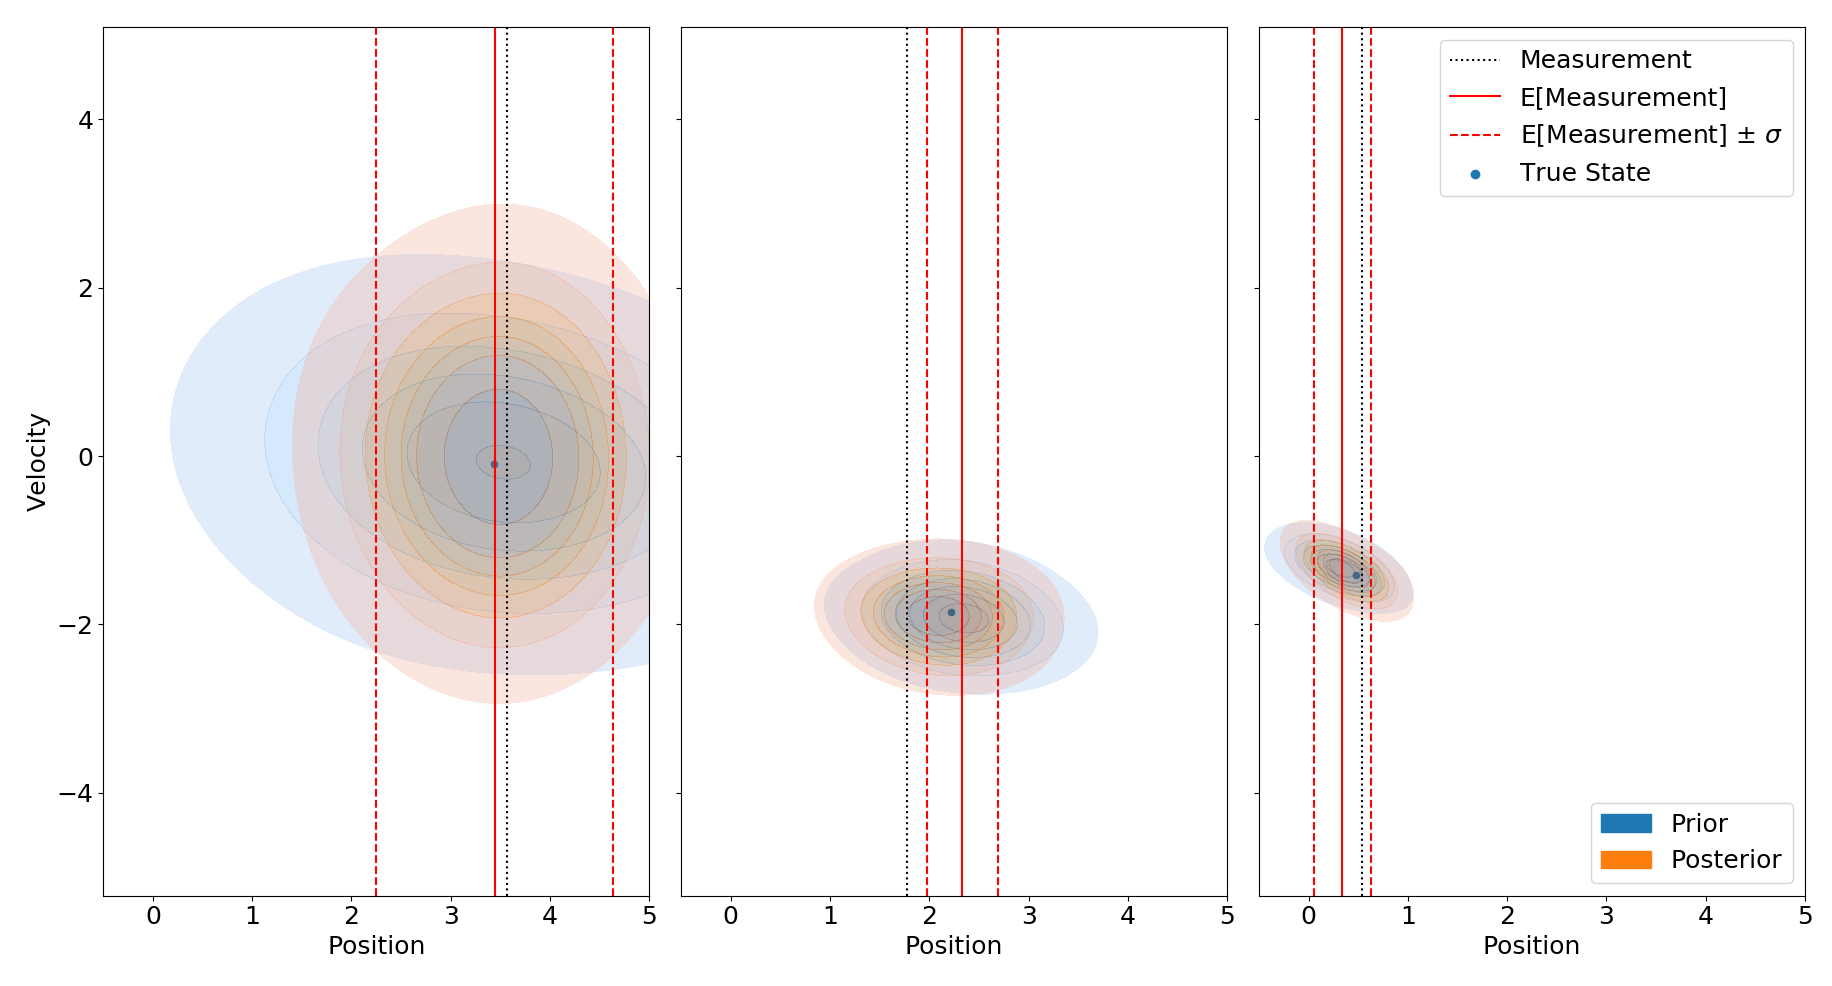
\includegraphics[width=\linewidth]{simulation_results.png}
    \label{simulation-results}
    \caption{Illustration of the category theoretic Kalman filter exhibiting the correct behavior for the model problem.}
\end{figure*}
\subsection{Problem Formulation}

We propose to 
Talk about the classical Kalman filter and the patterns that arise in the algorithm.

Talk about addressing this in a categorical framework.

\section{PROPOSED SOLUTION}

\subsection{General Framework}

In their book, Sussman and Abelson \cite{sicp} discuss at length techniques for creating powerful languages through abstraction.
We will follow their philosophy here.
While the devil is in the details, the overarching methodology is simple: programs should be seperated into \emph{layers} of absraction, and two layers will be tied together by a behavioral contract that each layer must follow. The lower layer should be more concrete and contain (possibly many) implementations of the contract, while the upper layer should be abstract and utilize the contract in algorithms.
These layers should be insulated from each other and communicate \emph{only} through the contract.
If there are multiple implementations of the contract in the concrete layer, the algorithms in the abstract layer should apply to all implementations as it simply has to communicate through the contract.

\subsubsection{Abstraction Example}

We take for example an extremely simple example where we want to abstract the concept of addition out of multiple types.
Say we want to create several data types that have the property that data can be added together to create new data.
For our contract, we shall create an Abstract Base Class called \texttt{Addable} that specifies that an addable type must have a built in method called \texttt{add\_us}.

\begin{listing}
\begin{minted}[
frame=lines,
framesep=2mm,
baselinestretch=1.2,
bgcolor=LightGray,
fontsize=\footnotesize,
]{python}
	class Addable(ABC):
		@abstractmethod
		def add_us(self, other): pass
\end{minted}
    \caption{Contract for specifying types must add}
\label{listing:1}
\end{listing}

The \texttt{@abstractmethod} decorator is a special decorator that forces any inheriting class to implement that method.
Thus, if a new datatype wants to inherit the \texttt{Addable} class, then the program will throw an error unless we specify an \texttt{add\_us()} method for that datatype.

Let's create a couple types: one will be our very own class for 2D vectors:

create vector code here

We implemented the \texttt{add\_us()} method to behave how one should expect (although there is unfortunately no way to force behavior to act as expect. We can only specify that the method must exist).
Now let's make a wrapper class for lists, where we simply want to express that lists can be added together through concatenation (pretending that this functionality doesn't already exist in python by default):

create concatenation code here

As of now we cannot do much, but we can use the method \texttt{add\_us} on two different types of data, and the method will do different things depending on what kind of data is passed.

show example of vectors and lists being added

While this is simple in concept, the power here lies on the fact that \emph{an abstract method in the contract that's called by a program will change its behavior based on its context.}
Here, we can start writing abstract programs that only make reference to the contract!
The first thing we'll do is exploit a language feature from Python: there exist certain special "underscore" methods that, when implemented, will allow you to start using infix operators.
In our case, implementing the \texttt{\_\_add\_\_()} method will give you usage of the \texttt{+} symbol.
So we will just write a simple wrapper that equivocates \texttt{\_\_add\_\_()} with \texttt{add\_us()}:

show wrapper function

We immediately get to start using + for both our types.

show usage

Next, we can write a simple generic function that only references the abstract method: a method called \texttt{double\_me()} which takes its input and doubles it under its own addition rules:

make double\_me

As we can see, we make no reference to vectors or lists in this code.
It is simply a 

\begin{listing}
\begin{minted}[
frame=lines,
framesep=2mm,
baselinestretch=1.2,
bgcolor=LightGray,
fontsize=\footnotesize,
]{python}
    def update(
        self, 
        dynamics, 
        instrument, 
        measurement
    ):
        prior = dynamics @ self
        updater = prior.bayes_invert(
            instrument
        )
        return updater @ measurement
\end{minted}
\caption{Category theoretic implementation of the classical Kalman Filter using our Python framework.}
\label{listing:1}
\end{listing}

Introduce algorithm with pseudocode.

\begin{listing}
\begin{minted}[
frame=lines,
framesep=2mm,
baselinestretch=1.2,
bgcolor=LightGray,
fontsize=\footnotesize,
]{python}
    class MarkovKernel(ABC):
	@abstractmethod
	def compose(f,g): pass

	@classmethod
	@abstractmethod
	def identity(X): pass

	@abstractmethod
	def product(f, g): pass

	@classmethod
	@abstractmethod
	def swapper(X,Y): pass

	@classmethod
	@abstractmethod
	def copier(X): pass

	@classmethod
	@abstractmethod
	def discarder(X): pass

	@abstractmethod
	def condition(f): pass
\end{minted}
    \caption{A (simplified) outline of the \texttt{MarkovKernel} abstract base class}
\label{listing:1}
\end{listing}

\begin{listing}
\begin{minted}[
frame=lines,
framesep=2mm,
baselinestretch=1.2,
bgcolor=LightGray,
fontsize=\footnotesize,
]{python}
    def update(
        self, 
        dynamics, 
        instrument, 
        measurement
    ):
        prior = dynamics @ self
        updater = prior.bayes_invert(
            instrument
        )
        return updater @ measurement
\end{minted}
\caption{Category theoretic implementation of the classical Kalman Filter using our Python framework.}
\label{listing:1}
\end{listing}


\begin{listing}
\begin{minted}[
frame=lines,
framesep=2mm,
baselinestretch=1.2,
bgcolor=LightGray,
fontsize=\footnotesize,
]{python}
    def bayes_invert(
        probability, 
        conditional
    ):
        return (
            conditional * probability
        ) / conditional.target
\end{minted}
\caption{Category theoretic implementation of Bayesian inversion using our Python framework.}
\label{listing:1}
\end{listing}

Probably use actual python to go over the language features used.

SHOW IMAGE OF STRING DIAGRAM ILLUSTRATING KALMAN FILTER

\begin{figure}[thpb]
    \framebox{\parbox{3in}{\centering\documentclass{standalone}
\usepackage{freetikz}
\begin{document}
\begin{tikzpicture}
    \centering
	\node[isosceles triangle,
	isosceles triangle apex angle = 60,
	draw,
	rotate = 270] (joint) at (1, 3) {\rotatebox{90}{$p$}};
	\node (xy) at (1,4) {$Y\otimes X$};

	\draw (joint.lower side) to[out=90, in=-90] (xy.south);
	\node (equals) at (2, 4) {$:=$};

	\node[isosceles triangle,
	isosceles triangle apex angle = 60,
	draw,
	rotate = 270] (xhat) at (3, 3) {\rotatebox{90}{$\hat{x}_{k-1}$}};

	\node[draw] (f) at (3, 4) {$f_{k-1}$};
	\node (copy) at (3, 4.5) {};
	\node[draw] (h) at (2.5, 5.5) {$h_{k}$};
	\node (y) at (2.5, 6.5) {$Y$};
	\node (x) at (3.5, 6.5) {$X$};

	\draw (xhat.lower side) to[out=90, in=-90] (f.south);
	\draw (f.north) to[out=90, in=-90] (copy.center);
	\draw (copy.center) to[out=180, in=-90] (h.south);
	\draw (h.north) to[out=90, in=-90] (y.south);
	\draw (copy.center) to[out=0, in=-90] (x.south);

\end{tikzpicture}
\end{document}
}}
    \label{propagate-string}
    \caption{Propagation step of the abstract filter}
\end{figure}

\begin{figure}[thpb]
    \framebox{\parbox{3in}{\centering\documentclass{standalone}
\usepackage{freetikz}
\begin{document}
\begin{tikzpicture}

	\node[isosceles triangle,
	isosceles triangle apex angle = 60,
	draw,
	rotate = 270] (xhat) at (0, 3) {\rotatebox{90}{$\hat{x}_{k}$}};

	\node (xnew) at (0,4) {$X$};
	\draw (xhat.lower side) to[out=90, in=-90] (xnew.south);

	\node at (1,4) {$:=$};
	
	\node[isosceles triangle,
	isosceles triangle apex angle = 60,
	draw,
	rotate = 270] (y) at (2, 3) {\rotatebox{90}{$y_k$}};

	\node[draw] (cond) at (2, 4) {$p_{|y}$};
	\node (x) at (2, 5) {$X$};

	\draw (y.lower side) to[out=90, in=-90] (cond.south);
	\draw (cond.north) to[out=90, in=-90] (x.south);
\end{tikzpicture}
\end{document}
}}
    \label{update-string}
    \caption{Update step of the abstract filter}
\end{figure}

then write it using infix notation

\section{SIMULATION RESULTS}

We demonstrate that the Kalman filter computed from the abstract formulation is identical to that implemented traditionally. 



\section{CONCLUSION}
It works.

\subsection{Future Work}

The software presented here is rudimentary, and thus there is still much work to be done in this field.
On top of the need to implement other representations of uncertainty, there is a plethora of absract formulations in this categorical context yet to be explored.

For the immediate future, we are working on representing Gaussian mixture transitions in this framework.

As a remark, there is a higher ordered sense of compositionality in these algorithms.

Gaussian Mixtures
Unscented Kalman filters/nonlinear stuff
Kalman filters on manifolds
Other abstract fomrulation such as stochastic control formulations.


%\section{PROCEDURE FOR PAPER SUBMISSION}
%
%\subsection{Selecting a Template (Heading 2)}
%
%First, confirm that you have the correct template for your paper size. This template has been tailored for output on the US-letter paper size. 
%It may be used for A4 paper size if the paper size setting is suitably modified.
%
%\subsection{Maintaining the Integrity of the Specifications}
%
%The template is used to format your paper and style the text. All margins, column widths, line spaces, and text fonts are prescribed; please do not alter them. You may note peculiarities. For example, the head margin in this template measures proportionately more than is customary. This measurement and others are deliberate, using specifications that anticipate your paper as one part of the entire proceedings, and not as an independent document. Please do not revise any of the current designations
%
%\section{MATH}
%
%Before you begin to format your paper, first write and save the content as a separate text file. Keep your text and graphic files separate until after the text has been formatted and styled. Do not use hard tabs, and limit use of hard returns to only one return at the end of a paragraph. Do not add any kind of pagination anywhere in the paper. Do not number text heads-the template will do that for you.
%
%Finally, complete content and organizational editing before formatting. Please take note of the following items when proofreading spelling and grammar:
%
%\subsection{Abbreviations and Acronyms} Define abbreviations and acronyms the first time they are used in the text, even after they have been defined in the abstract. Abbreviations such as IEEE, SI, MKS, CGS, sc, dc, and rms do not have to be defined. Do not use abbreviations in the title or heads unless they are unavoidable.
%
%\subsection{Units}
%
%\begin{itemize}
%
%\item Use either SI (MKS) or CGS as primary units. (SI units are encouraged.) English units may be used as secondary units (in parentheses). An exception would be the use of English units as identifiers in trade, such as .5-inch disk drive.
%\item Avoid combining SI and CGS units, such as current in amperes and magnetic field in oersteds. This often leads to confusion because equations do not balance dimensionally. If you must use mixed units, clearly state the units for each quantity that you use in an equation.
%\item Do not mix complete spellings and abbreviations of units: Wb/m2 or webers per square meter, not webers/m2.  Spell out units when they appear in text: . . . a few henries, not . . . a few H.
%\item Use a zero before decimal points: 0.25, not .25. Use cm3, not cc. (bullet list)
%
%\end{itemize}
%
%
%\subsection{Equations}
%
%The equations are an exception to the prescribed specifications of this template. You will need to determine whether or not your equation should be typed using either the Times New Roman or the Symbol font (please no other font). To create multileveled equations, it may be necessary to treat the equation as a graphic and insert it into the text after your paper is styled. Number equations consecutively. Equation numbers, within parentheses, are to position flush right, as in (1), using a right tab stop. To make your equations more compact, you may use the solidus ( / ), the exp function, or appropriate exponents. Italicize Roman symbols for quantities and variables, but not Greek symbols. Use a long dash rather than a hyphen for a minus sign. Punctuate equations with commas or periods when they are part of a sentence, as in
%
%$$
%\alpha + \beta = \chi \eqno{(1)}
%$$
%
%Note that the equation is centered using a center tab stop. Be sure that the symbols in your equation have been defined before or immediately following the equation. Use (1), not Eq. (1) or equation (1), except at the beginning of a sentence: Equation (1) is . . .
%
%\subsection{Some Common Mistakes}
%\begin{itemize}
%
%
%\item The word data is plural, not singular.
%\item The subscript for the permeability of vacuum ?0, and other common scientific constants, is zero with subscript formatting, not a lowercase letter o.
%\item In American English, commas, semi-/colons, periods, question and exclamation marks are located within quotation marks only when a complete thought or name is cited, such as a title or full quotation. When quotation marks are used, instead of a bold or italic typeface, to highlight a word or phrase, punctuation should appear outside of the quotation marks. A parenthetical phrase or statement at the end of a sentence is punctuated outside of the closing parenthesis (like this). (A parenthetical sentence is punctuated within the parentheses.)
%\item A graph within a graph is an inset, not an insert. The word alternatively is preferred to the word alternately (unless you really mean something that alternates).
%\item Do not use the word essentially to mean approximately or effectively.
%\item In your paper title, if the words that uses can accurately replace the word using, capitalize the u; if not, keep using lower-cased.
%\item Be aware of the different meanings of the homophones affect and effect, complement and compliment, discreet and discrete, principal and principle.
%\item Do not confuse imply and infer.
%\item The prefix non is not a word; it should be joined to the word it modifies, usually without a hyphen.
%\item There is no period after the et in the Latin abbreviation et al..
%\item The abbreviation i.e. means that is, and the abbreviation e.g. means for example.
%
%\end{itemize}
%
%
%\section{USING THE TEMPLATE}
%
%Use this sample document as your LaTeX source file to create your document. Save this file as {\bf root.tex}. You have to make sure to use the cls file that came with this distribution. If you use a different style file, you cannot expect to get required margins. Note also that when you are creating your out PDF file, the source file is only part of the equation. {\it Your \TeX\ $\rightarrow$ PDF filter determines the output file size. Even if you make all the specifications to output a letter file in the source - if your filter is set to produce A4, you will only get A4 output. }
%
%It is impossible to account for all possible situation, one would encounter using \TeX. If you are using multiple \TeX\ files you must make sure that the ``MAIN`` source file is called root.tex - this is particularly important if your conference is using PaperPlaza's built in \TeX\ to PDF conversion tool.
%
%\subsection{Headings, etc}
%
%Text heads organize the topics on a relational, hierarchical basis. For example, the paper title is the primary text head because all subsequent material relates and elaborates on this one topic. If there are two or more sub-topics, the next level head (uppercase Roman numerals) should be used and, conversely, if there are not at least two sub-topics, then no subheads should be introduced. Styles named Heading 1, Heading 2, Heading 3, and Heading 4 are prescribed.
%
%\subsection{Figures and Tables}
%
%Positioning Figures and Tables: Place figures and tables at the top and bottom of columns. Avoid placing them in the middle of columns. Large figures and tables may span across both columns. Figure captions should be below the figures; table heads should appear above the tables. Insert figures and tables after they are cited in the text. Use the abbreviation Fig. 1, even at the beginning of a sentence.
%
%\begin{table}[h]
%\caption{An Example of a Table}
%\label{table_example}
%\begin{center}
%\begin{tabular}{|c||c|}
%\hline
%One & Two\\
%\hline
%Three & Four\\
%\hline
%\end{tabular}
%\end{center}
%\end{table}
%
%
%   \begin{figure}[thpb]
%      \centering
%      \framebox{\parbox{3in}{We suggest that you use a text box to insert a graphic (which is ideally a 300 dpi TIFF or EPS file, with all fonts embedded) because, in an document, this method is somewhat more stable than directly inserting a picture.
%}}
%      %\includegraphics[scale=1.0]{figurefile}
%      \caption{Inductance of oscillation winding on amorphous
%       magnetic core versus DC bias magnetic field}
%      \label{figurelabel}
%   \end{figure}
%   
%
%Figure Labels: Use 8 point Times New Roman for Figure labels. Use words rather than symbols or abbreviations when writing Figure axis labels to avoid confusing the reader. As an example, write the quantity Magnetization, or Magnetization, M, not just M. If including units in the label, present them within parentheses. Do not label axes only with units. In the example, write Magnetization (A/m) or Magnetization {A[m(1)]}, not just A/m. Do not label axes with a ratio of quantities and units. For example, write Temperature (K), not Temperature/K.
%
%\section{CONCLUSIONS}
%
%A conclusion section is not required. Although a conclusion may review the main points of the paper, do not replicate the abstract as the conclusion. A conclusion might elaborate on the importance of the work or suggest applications and extensions. 
%
%\addtolength{\textheight}{-12cm}   % This command serves to balance the column lengths
%                                  % on the last page of the document manually. It shortens
%                                  % the textheight of the last page by a suitable amount.
%                                  % This command does not take effect until the next page
%                                  % so it should come on the page before the last. Make
%                                  % sure that you do not shorten the textheight too much.
%
%%%%%%%%%%%%%%%%%%%%%%%%%%%%%%%%%%%%%%%%%%%%%%%%%%%%%%%%%%%%%%%%%%%%%%%%%%%%%%%%%
%
%
%
%%%%%%%%%%%%%%%%%%%%%%%%%%%%%%%%%%%%%%%%%%%%%%%%%%%%%%%%%%%%%%%%%%%%%%%%%%%%%%%%%
%
%
%
%%%%%%%%%%%%%%%%%%%%%%%%%%%%%%%%%%%%%%%%%%%%%%%%%%%%%%%%%%%%%%%%%%%%%%%%%%%%%%%%%
%\section*{APPENDIX}
%
%Appendixes should appear before the acknowledgment.
%
%\section*{ACKNOWLEDGMENT}
%
%The preferred spelling of the word acknowledgment in America is without an e after the g. Avoid the stilted expression, One of us (R. B. G.) thanks . . .  Instead, try R. B. G. thanks. Put sponsor acknowledgments in the unnumbered footnote on the first page.
%
%
%
%%%%%%%%%%%%%%%%%%%%%%%%%%%%%%%%%%%%%%%%%%%%%%%%%%%%%%%%%%%%%%%%%%%%%%%%%%%%%%%%%
%
%References are important to the reader; therefore, each citation must be complete and correct. If at all possible, references should be commonly available publications.

\printbibliography

\end{document}
